\subsection{Problemas de información repetida}

Dentro de los problemas de información repetida, se encontraron los siguientes casos:

\begin{itemize}
\item[-] Tener información de una materia correspondiente a un plan de estudios posterior al semestre en el que se está buscando la información: \url{http://www.fciencias.unam.mx/docencia/horarios/20082/1556/803} y tener la misma información con el plan de estudios correspondiente: \url{http://www.fciencias.unam.mx/docencia/horarios/20082/218/803}

El número del plan de estudios corresponde al año en que entró en vigencia el plan. En la siguiente figura se puede ver una materia de la carrera de Ciencias de la Computación del semestre 2008-2, con planes distintos.


\begin{figure}[H]
	\centering
	\subfigure[Plan de estudios posterior]{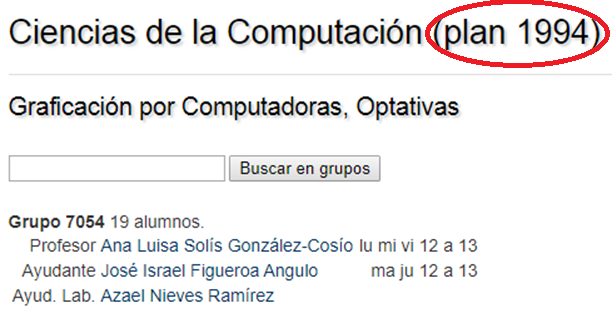
\includegraphics[width=7cm]{InfoRepetida_A_1}} %%Ping\"uino %%[angle=30]
	\subfigure[Plan de estudios correspondiente]{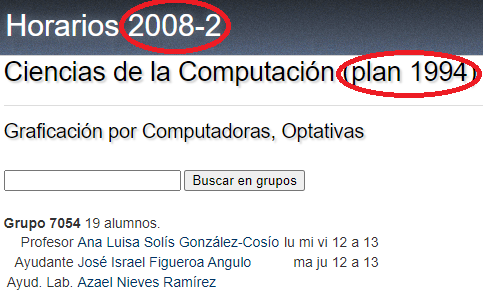
\includegraphics[width=7cm]{InfoRepetida_A_2}}
	\caption{\textit{Ejemplo de información repetida: Planes de estudio}}
\end{figure}

\item[-] Tener una misma materia con nombres distintos para las diferentes carreras: \url{http://www.fciencias.unam.mx/docencia/horarios/20201/217/1712} para Matemáicas, plan 1983 y \url{http://www.fciencias.unam.mx/docencia/horarios/20201/2017/1739} para Actuaría, plan 2015. Notamos que la información en ambas páginas es la misma, sólo se cambian las claves de los grupos.

\begin{figure}[H]
	\centering
	\subfigure[Matemáticas: 1983]{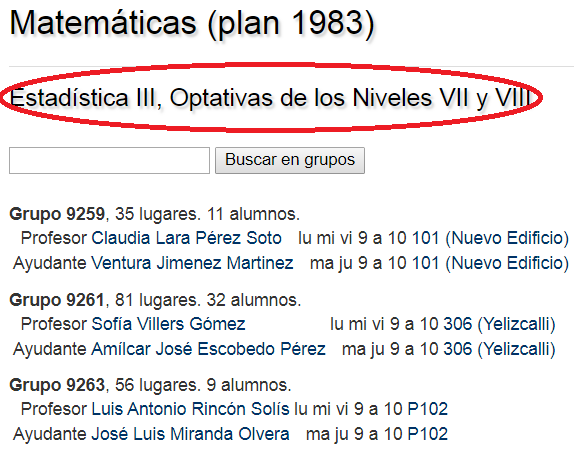
\includegraphics[width=6.5cm]{InfoRepetida_B_1}} %%Ping\"uino %%[angle=30]
	\subfigure[Actuaría: 2015]{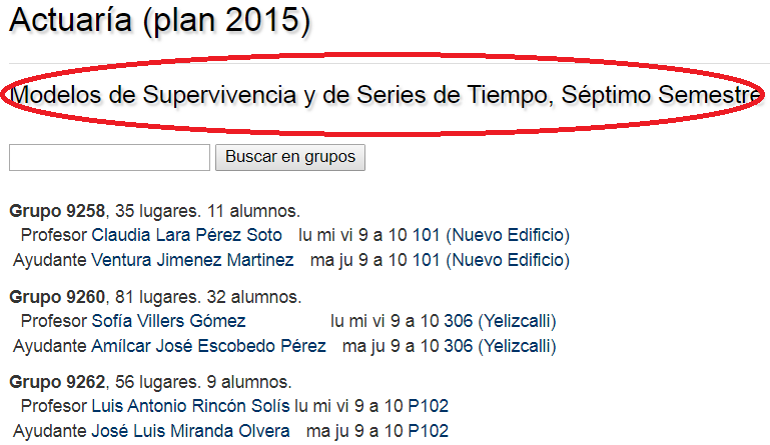
\includegraphics[width=7.5cm]{InfoRepetida_B_2}}
	\caption{\textit{Ejemplo de información repetida: Materia con nombres distintos}}
\end{figure}


\item[-] Profesores que imparten dos o más clases distintas en el mismo horario y diferente salón: \url{http://www.fciencias.unam.mx/docencia/horarios/20111/2017/162} para Ecuaciones Diferenciales I y \url{http://www.fciencias.unam.mx/docencia/horarios/20111/2017/91} para Cálculo Diferencial e Integral I.
  
Las materias mencionadas son diferentes, pero las clases comienzan a la misma hora, Ecuaciones de 18-19hrs y Cálculo de 18-20hrs, dado que se tiene la misma ayudante pudiera ser que se intercambien las horas, pero no se puede asignar más de una clase a la misma hora al mismo profesor.

\begin{figure}[H]
	\centering
	\subfigure[Ecuaciones Diferenciales I]{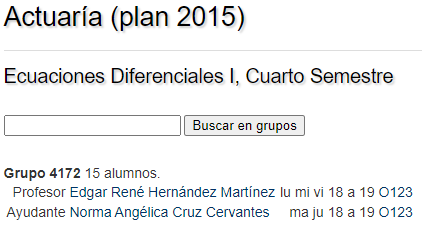
\includegraphics[width=10cm]{Ej_gpo_repetido_1}} %%Ping\"uino %%[angle=30]
	\subfigure[Cálculo Diferencial e Integral I]{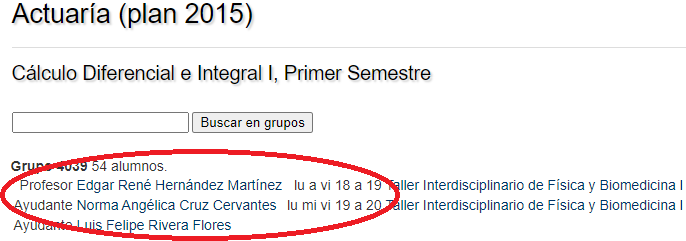
\includegraphics[width=15cm]{Ej_gpo_repetido_2}}
	\caption{\textit{Ejemplo de información repetida: Mismo profesor, materias distintas}}
\end{figure}	

%\begin{figure}[H]
%\centering
%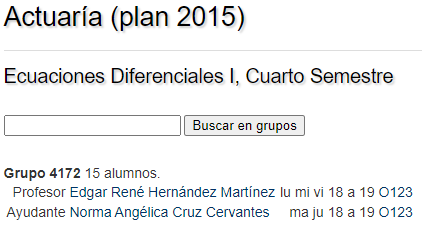
\includegraphics[scale = 0.65]{Ej_gpo_repetido_1} %width=\textwidth
%\caption{\textit{Ejemplo de grupo repetido (1)}}
%\end{figure}
%	
%\begin{figure}[H]
%\centering
%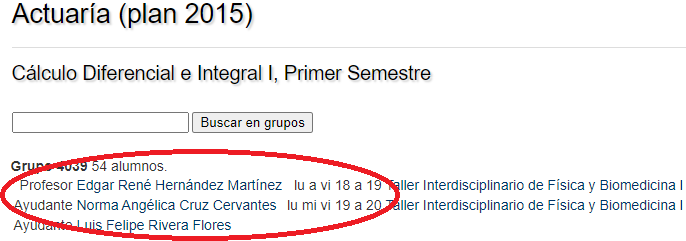
\includegraphics[scale = 0.65]{Ej_gpo_repetido_2} %width=\textwidth
%\caption{\textit{Ejemplo de grupo repetido (2)}}
%\end{figure}

%\begin{figure}[H]
%\centering
%\subfloat[Ecuaciones Diferenciales I]{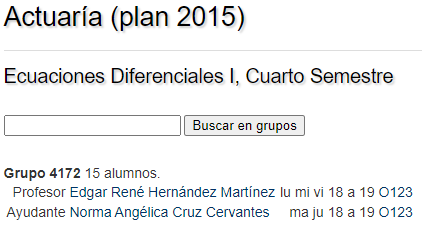
\includegraphics[width=0.3\textwidth]{Ej_gpo_repetido_1}}%[clip,width=\columnwidth]
%\subfloat[Cálculo Diferencial e Integral I]{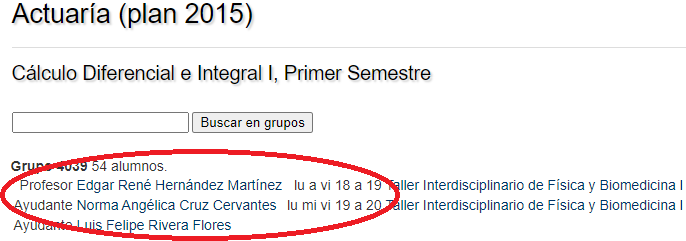
\includegraphics[width=0.3\textwidth]{Ej_gpo_repetido_2}}%[clip,width=0.6\columnwidth]
%\caption{\textit{Ejemplo de información repetida: Mismo profesor, materias distintas}}
%\end{figure}


\end{itemize}
